\documentclass[a4paper,11pt]{scrartcl}
\usepackage[left=2.5cm, right=3cm]{geometry}              % flexible and complete interface to document dimensions
\usepackage[latin1]{inputenc}                             % font encoding for umlauts
\usepackage[ngerman]{babel}                               % language settings
\usepackage[T1]{fontenc}                                  % T1 font encoding
\usepackage{amsmath}                                      % AMS mathematical facilities
%\usepackage{amssymb}                                     % defines symbol names for math symbols in the fonts MSAM and MSBM
\usepackage[bitstream-charter]{mathdesign}                % mathematical fonts to fit with Bitstream Charter
\usepackage{courier}                                      % replaces the current typewriter font for Adobe Courier
\usepackage{listings}                                     % source code printer
\usepackage{color}                                        % adding colors
\usepackage{fancyhdr}                                     % extensive control of page headers and footers
\usepackage{booktabs}                                     % publication quality tables
\usepackage{xcolor}                                       % driver-independent color extensions   
\usepackage{tikz}                                         % creating graphics programmatically
\usepackage{float}                                        % improved interface for floating objects
\usepackage{subfig}                                       % figures broken into subfigures
\usepackage{multirow}
\usepackage[linesnumbered,ruled,vlined]{algorithm2e}      % floating algorithm environment with algorithmic keywords

\definecolor{lightgray}{rgb}{.95,.95,.95}

\lstset{backgroundcolor=\color{lightgray},
        basicstyle=\ttfamily\fontsize{9pt}{9pt}\selectfont\upshape,
				commentstyle=\rmfamily\slshape,
				keywordstyle=\rmfamily\bfseries\color{black},
				captionpos=b,
				showstringspaces=false,
				breaklines=true,
				frame=lines,
				tabsize=2,
				aboveskip={\baselineskip}
}

\renewcommand{\labelenumi}{(\arabic{enumi})}
\renewcommand{\labelenumii}{(\alph{enumii})}
\renewcommand{\algorithmcfname}{Algorithmus}

\subject{Dokumentation}
\title{XML Technologien Projekt}
\author{David Bialik $\cdot$ Kevin Funk\\ Jan Kostulski $\cdot$ Konrad Reiche $\cdot$ Andr� Zoufahl}
\date{\today}
\publishers{\vskip 2ex -- Gruppe 3 --}

\begin{document}

\pagestyle{fancy}
\maketitle

\section{Einleitung}

Dieses Dokument beschreibt die L�sung des Softwareprojekts f�r den Kurs XML Technologien Sommersemester 2012 bearbeitet von Gruppe 3. Aufgabenstellung war es �ber den Dienst \emph{gpsies.com} Informationen �ber verschiedene Routen in Form von XML Dokumenten zu beschaffen, diese unter Nutzung von semantischer Anreicherung zu erweitern und schlussendlich auf einer selbst entwickelten Weboberfl�che anzubieten.

Im weiteren werden wir auf Implementierungsdetails eingehen, erl�utern welche Probleme aufgetreten sind und deren L�sungen diskutieren. Am Ende gibt es eine Anleitung zur Verwendung der Anwendung. Zun�chst wird die Systemarchitektur unserer L�sung skizziert.

\section{Systemarchitektur}

Die Systemarchitektur ist in Abbildung \ref{fig:architecture} skizziert. An ihr kann auch der Ablauf der Anwendung erl�utert werden:

\begin{enumerate}
\item der Crawler, als unabh�ngige Komponente, wird in zwei Schritten ausgef�hrt

\begin{enumerate}
\item laden der \emph{Result Pages} von gpsies.org und Persistieren auf der XML Datenbank

\item laden der \emph{Track Details} pro \emph{File Id} von gpsies.org und Persistieren auf der XML Datenbank
\end{enumerate}

\item das SPARQL Skript, ebenfalls als unabh�ngige Komponente, konstruiert pro Track 2 SPARQL Queries (Anfangs- und Endkoordinaten) und sendet diese Anfrage an DBpedia, die Antwort wird als JSON bearbeitet und als Erweiterung in die XML Datenbank zur�ckgeschrieben

\item der Web Server sendet auf Anfrage durch den Benutzer das HTML Formular f�r eine detaillierte Suche in den Tracks, dabei wird die HTML Seite mithilfe von XSLT konstruiert.

\item auf Suchanfrage durch den Benutzer werden entsprechende Dokumente durch XQuery Anfrage an die Datenbank geladen, Point of Interest Daten werden verwendet um Zusatzinformationen vom Kurznachrichtendienst Twitter zu erhalten, beim Konstruieren des HTML Ergebnis wird Microdata zur semantischen Erweiterung hinzugef�gt.

\end{enumerate}

\begin{figure}[H]
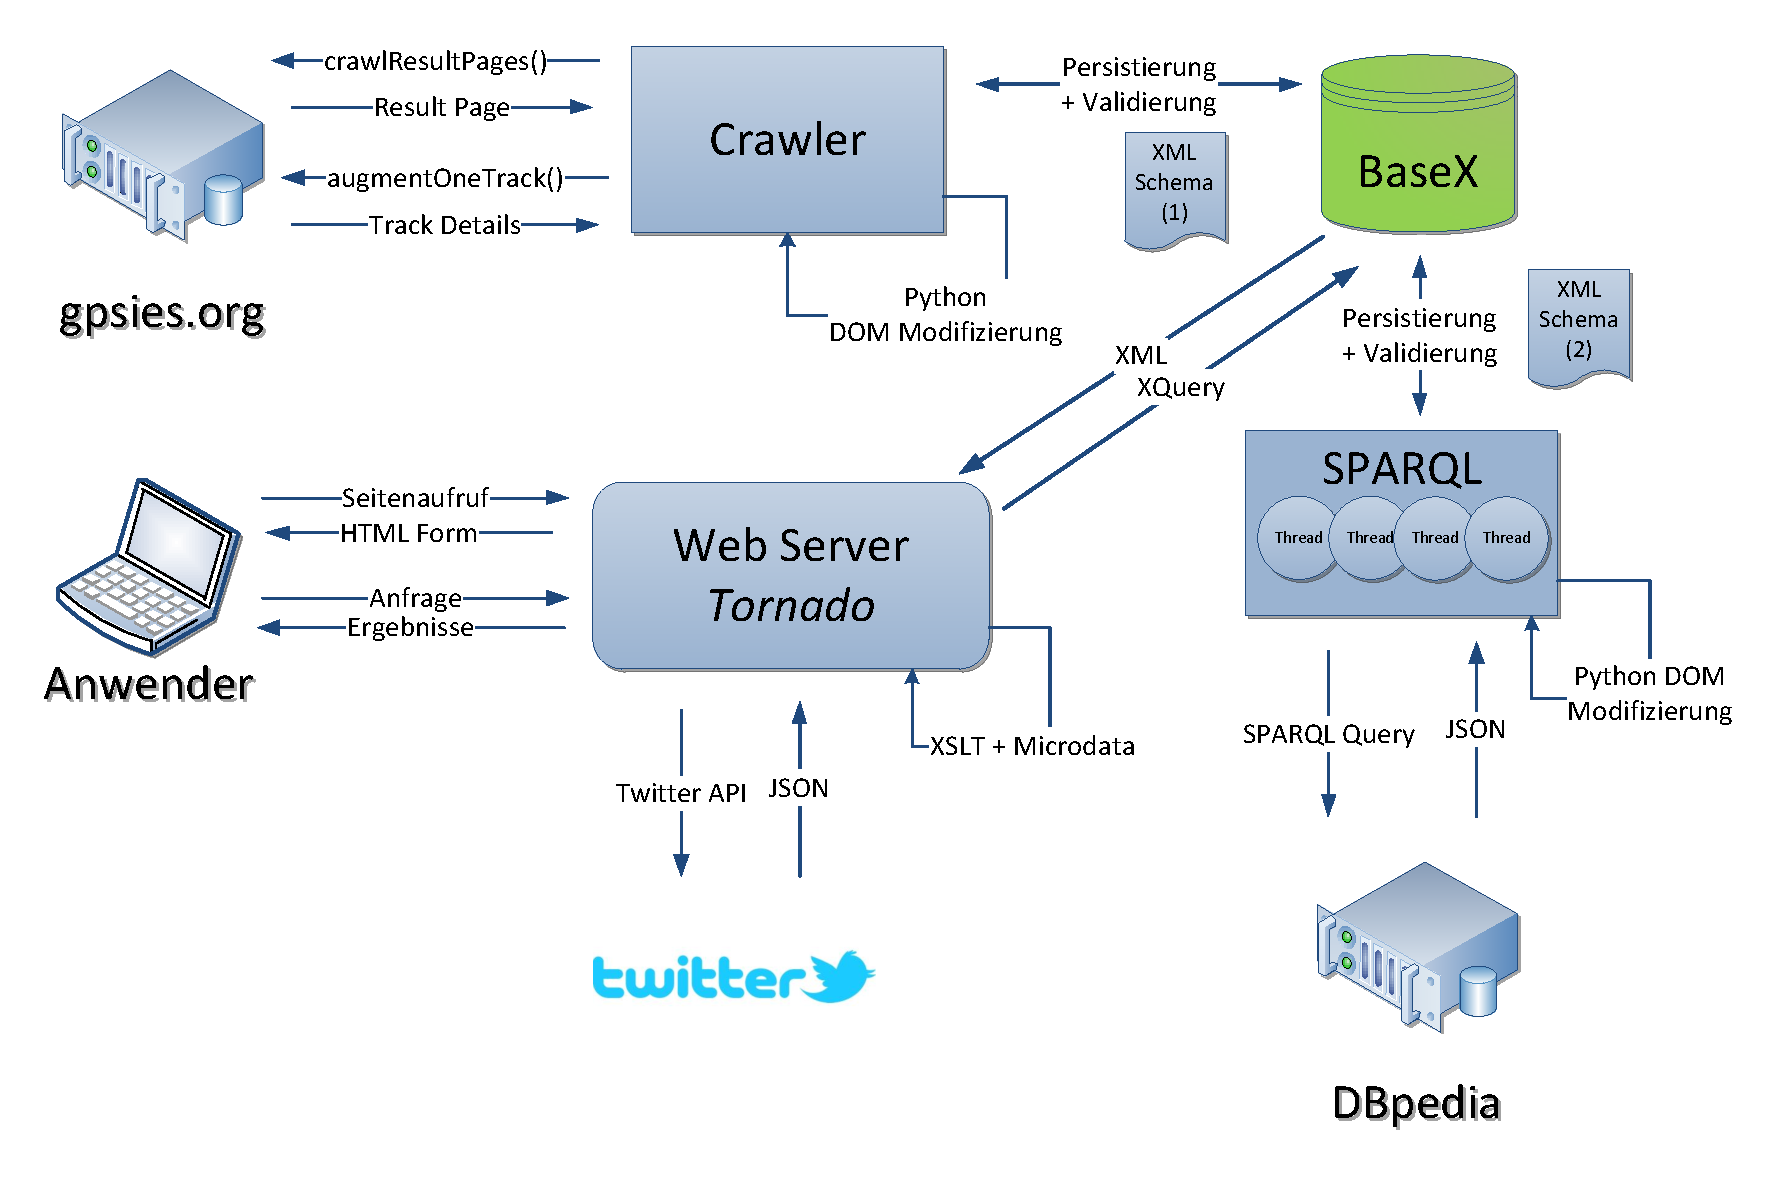
\includegraphics[width=\columnwidth]{resources/architecture.pdf}
\caption{Skizze der Architektur mit den verschiedenen Komponenten und Interaktionen}
\label{fig:architecture}
\end{figure}

Jeder Track wird als einzelnes Dokument in der XML Datenbank abgelegt. Es gibt zwei Validierungsschritte, zum einen die Validierung der Trackdokumente nach einem Schema wie sie von \emph{gpsies.org} direkt ausgeliefert werden und zum anderen das XML Schema nach der augmentierung durch das SPARQL Skript. F�r das SPARQL Skript wurden mehrere Threads verwendet um mehrere Tracks gleichzeitig zu erweitern.

\section{Implementierung}

\subsection{Crawler}

Das Script \emph{crawler.py} umfasst folgende Funktionen

\begin{lstlisting}
usage: crawler [-h] [-c] [-e] [-s] [-p]

XML Crawler for gpsies.com

optional arguments:
  -h, --help        show this help message and exit
  -c, --crawl       Crawl from gpsies.com, parse result pages
  -e, --extend      Crawl from gpsies.com, extend non-augmented tracks with
                    track details
  -s, --statistics  Print database statistics
  -p, --prune       Clear database, remove all non-augmented tracks
\end{lstlisting}

Der Crawler implementiert zwei Hauptaktionen (\emph{crawl, extend}), um die Datenbank mit XML-Daten von \emph{gpsies.org} zu f�llen.

\subsubsection{Crawl}
\begin{itemize}
  \item Es werden Resultpages mit jeweils 100 Tracks von \emph{gpsies.org} abgefragt
\footnote{Beispiel-URL: http://www.gpsies.org/api.do?key=API\_KEY\&country\=DE\&limit=100\&resultPage=1}
  \item Davon werden die einzelnen \emph{<track/>}-Elemente geparst
  \item Diese werden einzeln als Dokument in die Datenbank geschrieben
  \item Der Dokumentenname ist hierbei die Track-FileID
\end{itemize}

\subsubsection{Extend (Augment)}
\begin{itemize}
  \item Hier werden sukzessiv nicht-augmentierte Tracks aus der Datenbank angereichert
  \item Pro Track werden die Trackdetails von \emph{gpsies.org} geholt
\footnote{Beispiel-URL: http://www.gpsies.org/api.do?key=API\_KEY\&fileId=cimmxugjixiyzakj\&trackDataLength=250}
  \item Danach wird der Track durch die detaillreichere Version in der Datenbank ersetzt
\end{itemize}

\subsection{SPARQL-Abfrage}

% TODO: Konrad

\subsection{Webserver}

% TODO: Kevin, Andre

\section{Test-Umgebung}

\subsection{Referenzsystem}

Unsere Anwendunge wurde haupts�chlich auf folgender Plattform getestet:

\begin{itemize}
  \item Ubuntu 12.04

  \begin{itemize}
    \item Python 2.7.3
    \item BaseX 7.0.2
  \end{itemize}
\end{itemize}

\subsection{Tests}

% TODO: Kevin

\section{Installationsanleitung}

\subsection{Abh�ngigkeiten}

\begin{itemize}
  \item BaseX (http://basex.org/)
  \item Tornado Web Server (http://www.tornadoweb.org/)
  \item Python LXML (http://lxml.de)
  \item SPARQL Endpoint interface to Python (http://sparql-wrapper.sourceforge.net/)
\end{itemize}

\subsubsection{Quick install (f�r Debian-basierte Systeme)}

Getestet auf Ubuntu 12.04.

\begin{lstlisting}
* apt-get install basex python-tornado python-lxml python-sparqlwrapper
\end{lstlisting}


\subsection{Datenbank aufsetzen}

% TODO: Woher Datenbankdump
Zun�chst muss der Datenbankdump (\emph{default-*.zip}) nach \emph{\$HOME/BaseXData/} kopiert werden um sie sp�ter importieren zu k�nnen.

Starten der BaseX-Datenbank

\begin{lstlisting}
$ basexserver
\end{lstlisting}

Erstmaliges Erstellen der Datenbank

\begin{lstlisting}
$ basexclient

# Notiz: Der Standardlogin ist admin:admnin

$ > create database default
\end{lstlisting}

Importieren unseres Datenbankdumps:
\begin{lstlisting}
$ > restore default
\end{lstlisting}

\subsection{Ausf�hren des Crawlers (optional)}

Zum Ausf�hren des Crawlers muss eine Internetverbindung bestehen und die Verf�gbarkeit von \emph{gpsies.org} gew�hrleistet sein.
Au�erdem muss eine BaseX-Server-Instanz f�r die Datenbankanbindung laufen.

Danach kann der Crawler folgenderma�en gestartet werden:
\footnote{Notiz: Alle ausf�hrbaren Dateien liegen im Projektorder \emph{src/}}

\begin{lstlisting}
# Parse result pages from gpsies.org
$ ./crawler.py -c
\end{lstlisting}

Der Crawler l�uft mit diesem Parameter solange, bis er mindestens $100000$ Tracks in der Datenbank gespeichert hat. Diesen Tracks fehlen dann aber noch Detaillinformationen, wie die Startpunktaddresse, welche aber f�r die Suchmaske auf dem Webformular gebraucht werden.

Um diese Informationen zu bekommen muss danach der Crawler mit folgenden Parameters gestartet werden.

\begin{lstlisting}
# Augment tracks with information from gpsies.org
$ ./crawler.py -e
\end{lstlisting}

Bei diesem Aufruf fragt der Crawler f�r jeden Track in der Datenbank die Detaillinformationen auf \emph{gpsies.org} ab und reichert damit die jeweiligen Tracks an.

\subsection{Anreicherung mit Point-Of-Interests (optional)}

% TODO: Konrad?

\subsection{Webserver starten}

Nachdem die Datenbank bef�llt ist, kann der Webserver gestartet werden.

\begin{lstlisting}
# Start web server
$ ./web.py
\end{lstlisting}

Dies startet einen Tornado-Webserver auf der Adresse \emph{http://localhost:8888} welche mit dem Browser angesteuert werden kann.

\section{Benutzerdokumentation}

\end{document}
